\documentclass[12pt,notitlepage,oneside]{report}
\setcounter{secnumdepth}{3}
\usepackage{buet_msc_thesis}
\usepackage{lipsum}
\usepackage{svg}
%\usepackage[acronym, toc]{glossaries}

% Uncomment any of the following lines should you need to
% suppress the LOF, or LOT or LOA

% \suppresslistoffigures 
% \suppresslistoftables
% \suppresslistofalgorithms

%parameters for thesis

% Please make sure that the title is EXACTLY same
% as the one passed in the CASR meeting.
% Please ask your supervisor for a copy of the 
% CASR meeting resolutioin before typing below
\def\thesistitle{Put the Title of Your Thesis Here}
% the Date below is the date of the final examination (month and year).

\def\thesisdefenseday{15}
\def\thesisdefensemonthyear{September  2020}
\def\author{Candidate Name}
\def\StudentID{042106XYZA}
\def\degree{Master of Science}
\def\department{Department of Electrical and Electronic Engineering}
\def\subject{Electrical and Electronic Engineering}
\def\session{April 2021}
\def\deptaffiliation{Department of EEE, BUET, Dhaka}

% For index creation, comment this out if you do not want to create an
% index
\makeindex[intoc]
\patchcmd{\titlepage}{empty}{fancy}{}{}
\patchcmd{\chapter}{plain}{fancy}{}{}

\begin{document}


% Edit as needed below this line
% %%%%%%%%%%%%%%%%%%%%%%%%%%%%%%%%%%%%%%%%%%%%%%%%%%%%%%%%
% Chapter-1

\chapter{Introduction}\label{intro}

Filename: chapters/introduction.tex
The following sections are examples.
\section{Problem Statement}
Section text. Figure~\ref{fig:example}.
\begin{figure}
	\centering {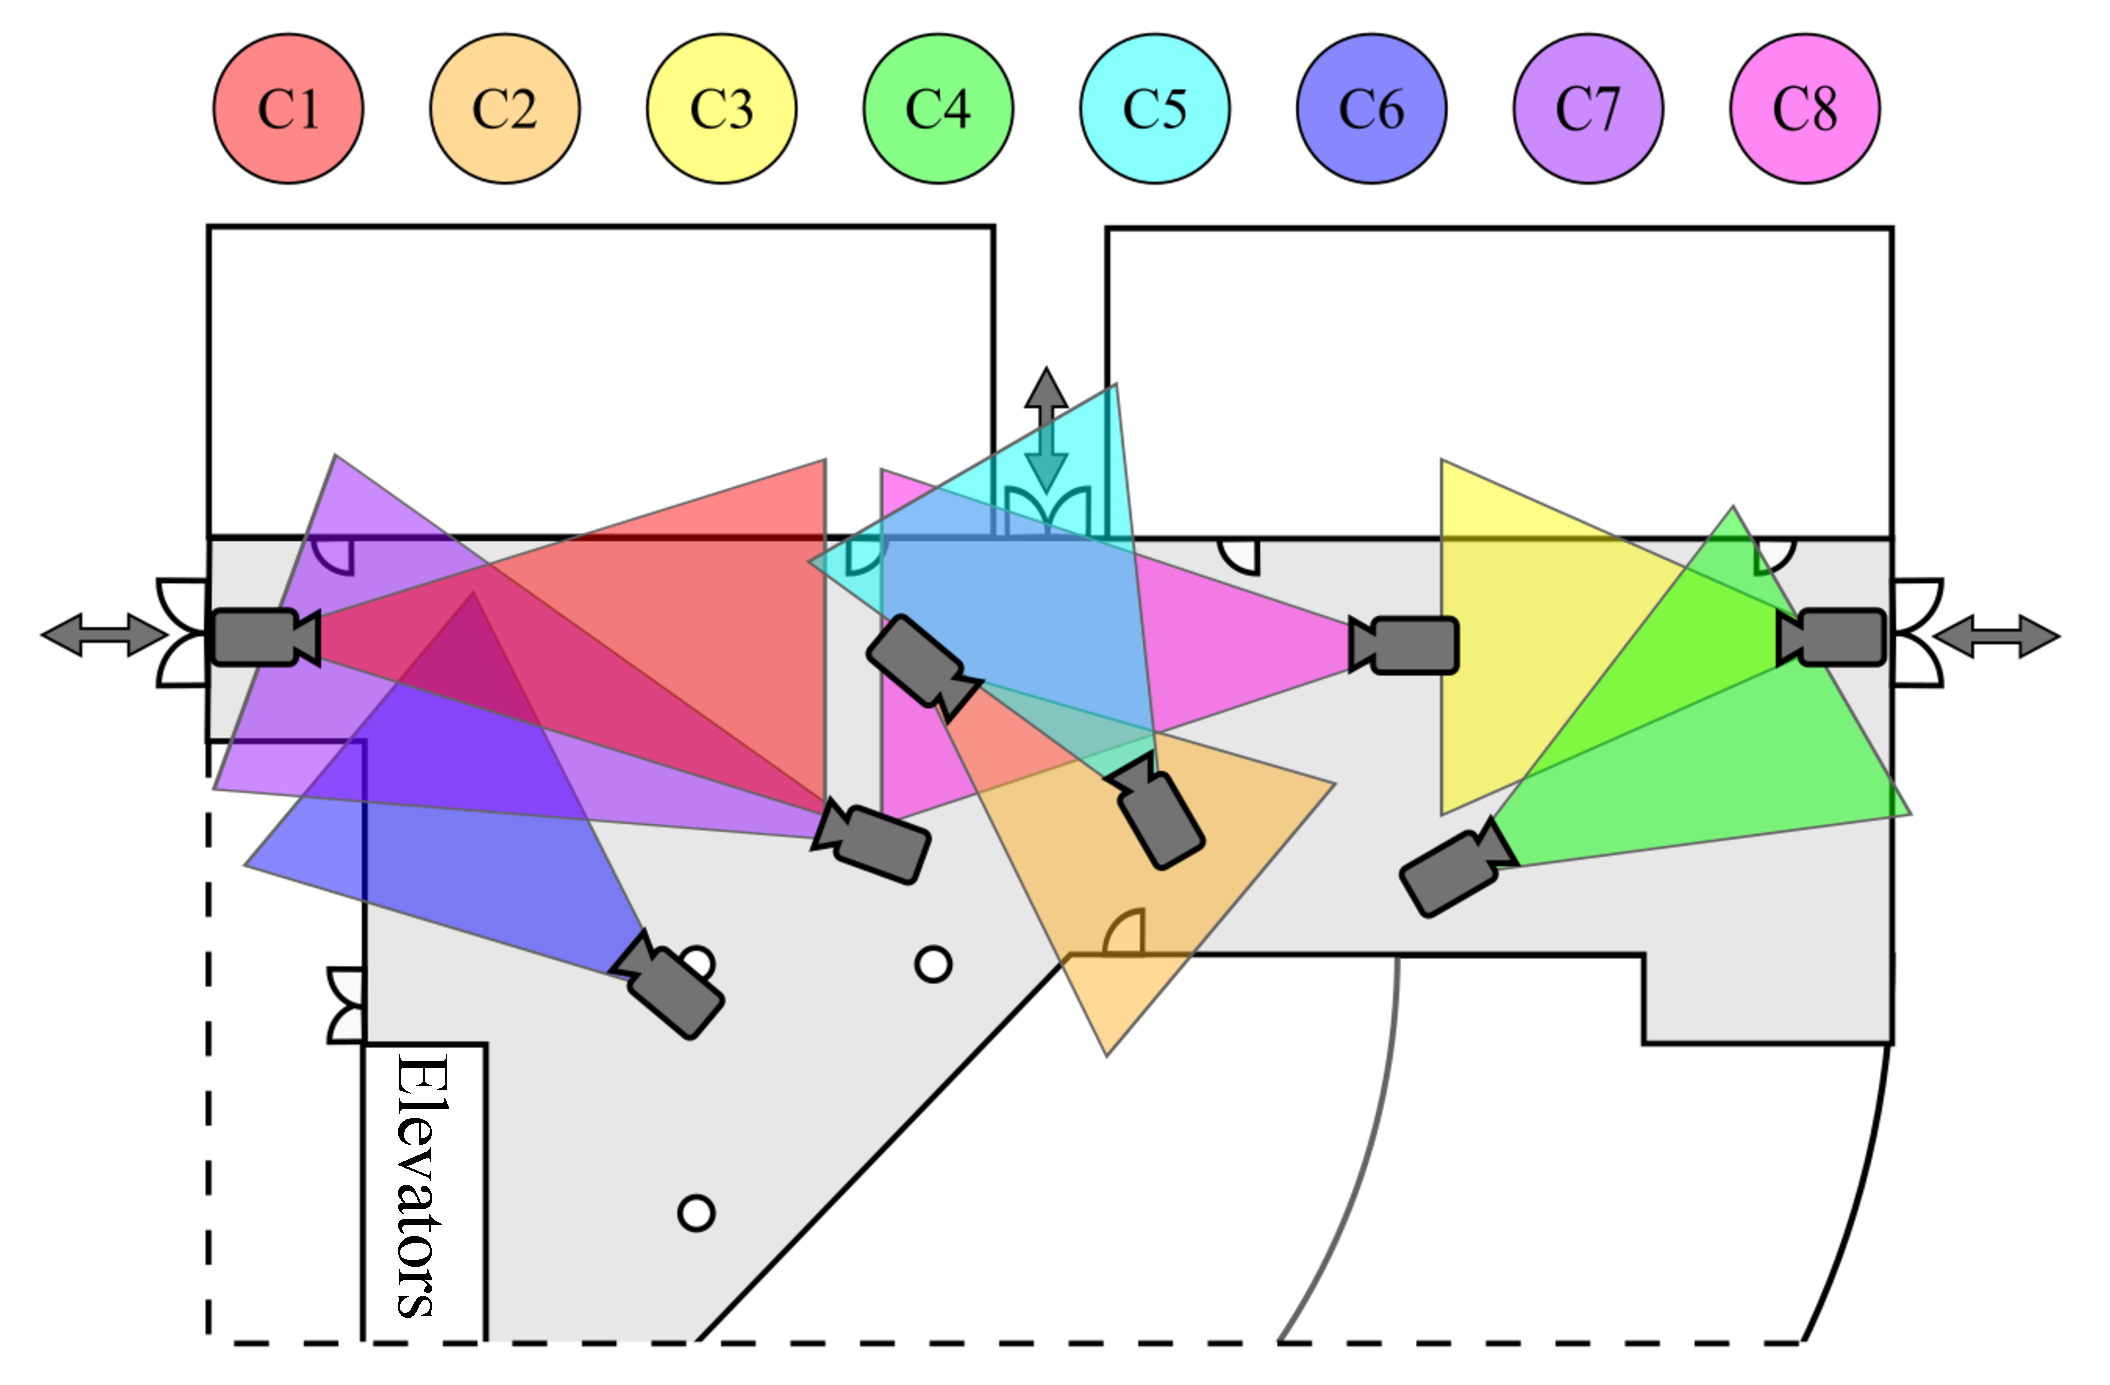
\includegraphics[width=0.7\textwidth]{figures/figure1.eps}}
	\caption
	{Example Figure \label{fig:example}}
\end{figure}


\section{Objectives of the Thesis}
From the proposal

\section{Thesis Outline} 
The rest of this thesis is organized as follows.

% Chapter-2
\chapter{Literature Review} \label{ch:literature_review}
Filename: chapters/literature\_review.tex

Literature review chapter. Citation example~\cite{Rida_19}.

Add the references in buet\_msc\_thesis.bib files in bibtex format.

 




% Chapter-3
\chapter{Background}
\label{ch:background}
Filename: chapters/background.tex

Background chapter. Add sections as necessary.




% Chapter-4
\chapter{Proposed  System} \label{ch:methodology}
Filename: chapters/methodology.tex

In this chapter, we discuss the proposed system...  


\begin{table}
	\centering
	\caption{Example Table \label{table:summary_tn}}
	\begin{tabular*}{32pc}{@{\extracolsep{\fill}}ll@{}}
		\hline \noalign{\vspace{3pt}}
		\textbf{Hyperparameter} &\qquad \textbf{Value} \\ [3pt] \hline\noalign{\vspace{3pt}}
		Optimizer     			&\qquad Adam~\cite{Kingma_15} \\[3pt]
		Objective function  	&\qquad Fusion of softmax and center loss \\[3pt]
		Epochs        			&\qquad $ 450 $ \\ [3pt]
		Initial learning rate	&\qquad $5 \times 10^{-3}$  \\[3pt]
		Mini-batch size			&\qquad $ 256 $ \\
		\hline
	\end{tabular*}
\end{table}



% Chapter-5
\chapter{Experimental Results}\label{ch:experimental_result}
Filename: chapters/result\_discussion.tex

In this chapter, we are going to evaluate our proposed method ...

% Chapter-6
\chapter{Conclusions}\label{ch:conclusion}
Filename: chapters/conclusion.tex
\section{Conclusions}


\section{Future Prospects of Our Work}



% Chapter showing example of index creation
%\chapter{Index Creation}
\section{BUET}
Bangladesh University of Engineering and Technology, abbreviated as
BUET\index{BUET}, is one of the most prestigious institutions for
higher studies in the country. About 5500 students are pursuing
undergraduate\index{BUET!undergraduate} and
postgraduate\index{BUET!postgraduate} studies in engineering,
architecture, planning and science in this institution. At present,
BUET has sixteen teaching departments under five faculties and it has
three institutes. Every year the intake of undergraduate students is
around 900, while the intake of graduate students in Master's and PhD
programs is around 1000. A total of about five hundred teachers are
teaching in these departments and institutes. There are additional
teaching posts like Dr.\ Rashid Professor, Professor Emeritus and
Supernumerary Professors.
 
\section{Campus}
The BUET campus is in the heart of Dhaka\index{Dhaka} --- the capital
city of Bangladesh. It has a compact campus with halls of residence
within walking distances of the academic buildings. The physical
expansion of the University over the last three decades has been
impressive with construction of new academic buildings,
auditorium\index{BUET!auditorium} complex, halls of residence, etc.
 
\section{History}\index{BUET!History}
BUET is the oldest institution for the study of Engineering and
Architecture in Bangladesh. The history of this institution dates back
to the days of Dhaka Survey School which was established at
Nalgola\index{Nalgola}, in Old Dhaka in 1876 to train Surveyors for
the then Government of Bengal of British India. As the years passed,
the Survey School became the Ahsanullah School of
Engineering\index{Ahsanullah School of Engineering} offering
three-year diploma courses in Civil, Electrical and Mechanical
Engineering. In recognition of the generous financial contribution
from the then Nawab of Dhaka, it was named after his father Khawja
Ahsanullah. It moved to its present premises in 1912. In 1947, the
School was upgraded to Ahsanullah Engineering College as a Faculty of
Engineering under the University of Dhaka, offering four-year
bachelor’s courses in Civil, Electrical, Mechanical, Chemical and
Metallurgical Engineering. In order to create facilities for
postgraduate studies and research, Ahsanullah Engineering College was
upgraded to the status of a University in 1962 and was named East
Pakistan University of Engineering and Technology. After the War of
Liberation in 1971\index{1971|see {War of Liberation}}\index{War of
  Liberation}, Bangladesh became an independent state and the
university was renamed as the Bangladesh University of Engineering and
Technology.
 
\section{Students}
Till today, it has produced around 25,000 graduates in different
branches of engineering and architecture, and has established a good
reputation all over the world for the quality of its graduates, many
of whom have excelled in their profession in different parts of the
globe. It was able to attract students from countries like
India\index{India}, Nepal\index{Nepal}, Iran\index{Iran},
Jordan\index{Jordan}, Malaysia\index{Malaysia}, Sri Lanka\index{Sri
  Lanka}, Pakistan\index{Pakistan} and Palestine\index{Palestine}.
 
\section{Departments}
Both Undergraduate and Postgraduate studies and research are now among
the primary functions of the University. Eleven departments under five
faculties offer Bachelor Degrees, while most of the departments and
institutes offer Master's Degrees and some of the departments have
Ph.D. programs. In addition to its own research programs, the
university undertakes research programs sponsored by outside
organizations like European Union, UNO,
Commonwealth\index{Commonwealth}, UGC\index{UGC}, etc. The expertise
of the University teachers and the laboratory facilities of the
University are also utilized to solve problems and to provide
up-to-date engineering and technological knowledge to the various
organizations of the country.


\endinput


% Bibliographies and appendices
% You do not need to change anything in this file. If you want to
% change the reference style, comment/uncomment the \bibliographystyle
% lines

\clearpage
\renewcommand\bibname{References}
\addcontentsline{toc}{chapter}{\textbf{References}}

% Comment/uncomment as suits you
\bibliographystyle{BUET} %% BUET  style
% \bibliographystyle{IEEEtran} %% IEEE transaction style
% \bibliographystyle{acm} %% ACM style
% \bibliographystyle{alpha}


\bibliography{buet_msc_thesis}
%\addbibresource{buet_msc_thesis.bib}
\endinput


% Index, comment this out if you do not want to create an index
\printindex

\appendix
% Algorithms
%\input{chapters/algorithms.tex}

\end{document}